\section{Results}
\subsection{PE-RankFormer combines edit-aware sequence modeling with ordinal supervision}
\model{} represents each candidate through two complementary sequence streams: aligned wild-type/edited nucleotide pairs describe the intended edit, and a segment-aware pegRNA stream describes the spacer, PBS and RTT. Bidirectional cross-attention integrates these representations, and FiLM conditioning incorporates experimental metadata (Figure~\ref{fig:architecture}). The ordinal head learns a set of cumulative outcome thresholds and averages their predicted exceedance probabilities to obtain a ranking score (Equation~\ref{eq:ordinal}). This score is order-sensitive but need not be an absolute-efficiency estimate; the loss does not directly optimize sample Spearman correlation.

We evaluated Transformer and bidirectional S4D encoders and ordinal and proportion-based heads. The frozen source-benchmark system combines five families, each represented by five official-fold checkpoints. External zero-shot evaluation uses the five-fold ordinal--S4D family, while the supported target-adaptation procedure fine-tunes a predetermined single checkpoint from that family. We distinguish these configurations rather than treating the ensemble and adapted backbone as an identical deployed model. Adaptation retains the native ordinal head and updates selected encoder/readout modules; it requires neither a separate selection branch nor OptiPrime-derived information. Model details are given in Methods, and evaluation populations and exposure histories in Supplementary Table~\ref{tab:populations}.

\begin{figure}[htbp]
\centering
\begin{tikzpicture}[node distance=8mm,box/.style={draw,rounded corners,align=center,text width=4.4cm,minimum height=10mm,font=\small},arr/.style={-{Latex},thick}]
\node[box] (edit) {Aligned wild-type/edited pairs\\edit encoder (6 blocks)};
\node[box,right=12mm of edit] (peg) {Spacer, PBS and RTT with segment identity\\pegRNA encoder (4 blocks)};
\node[box,below=of edit,xshift=2.8cm,text width=6cm] (cross) {Bidirectional cross-attention (2 blocks)\\pooling and experimental-context conditioning};
\node[box,below=of cross,text width=6cm] (source) {Order-sensitive source training\\ordinal thresholds / complementary proportion heads};
\node[box,below=of source,xshift=-2.6cm,text width=4.3cm] (rank) {Source-trained scoring\\benchmark and external ranking};
\node[box,right=8mm of rank,text width=4.3cm] (adapt) {Target-library fine-tuning\\native ordinal head, selected blocks};
\node[box,below=of rank,text width=4.3cm] (selectsource) {Source-domain selection\\highest-scored pegRNA per edit};
\node[box,below=of adapt,text width=4.3cm] (selecttarget) {Target-domain selection\\highest-scored pegRNA per edit};
\draw[arr] (edit.south)--(cross.north west);
\draw[arr] (peg.south)--(cross.north east);
\draw[arr] (cross)--(source);
\draw[arr] (source.south)--(rank.north);
\draw[arr] (source.south)--(adapt.north);
\draw[arr] (rank)--(selectsource);
\draw[arr] (adapt)--(selecttarget);
\end{tikzpicture}
\caption{\textbf{\model{} integrates edit-aware representation learning with pegRNA ranking and selection.} Self-attention or bidirectional S4D mixes tokens within each stream; cross-attention connects guide and target. The source ensemble combines ordinal and proportion-based families. External zero-shot ranking uses the five-fold ordinal--S4D ensemble, whereas target fine-tuning starts from a predetermined single ordinal--S4D checkpoint and retains its native score. These are distinct configurations of the framework. No OptiPrime predictions or parameters enter the model. The supplementary adaptation experiments test additional selector and preservation variants, not required components of the main method.}
\label{fig:architecture}
\end{figure}


\subsection{PE-RankFormer outperforms OptiPrime across source rank-based metrics}
The source corpus comprises 318,471 measurements, with 297,962 training/development rows and 20,509 official held-out rows. The held-out benchmark includes 9,175 Liu-derived and 11,334 Kim-derived measurements.
On the original held-out benchmark, the frozen heterogeneous \model{} ensemble reached \rhoS{} $=0.9079$, compared with $0.8690$ for released OptiPrime (Figure~\ref{fig:prediction}; Table~\ref{tab:source}). The paired difference was $+0.0389$, with the original 5,000-resample protospacer bootstrap interval $[+0.0286,+0.0498]$. The difference was larger in Kim-derived records than in Liu-derived records. Within 14 sufficiently populated source/cell/editor conditions, the row-weighted average correlation was $0.8111$ versus $0.7605$, a difference of $+0.0506$ with interval $[+0.0345,+0.0670]$. The gain therefore does not disappear when between-condition differences are removed.

\begin{table}[htbp]
\centering\small
\caption{PE-RankFormer outperforms OptiPrime across source rank-based metrics.}
\label{tab:source}
\begin{tabular}{lrrr}
\toprule
Endpoint & OptiPrime & \model{} & Difference \\
\midrule
Pooled Spearman, 20,509 rows & 0.8690 & 0.9079 & +0.0389 \\
Liu Spearman, 9,175 rows & 0.8365 & 0.8585 & +0.0220 \\
Kim Spearman, 11,334 rows & 0.7320 & 0.8124 & +0.0803 \\
Within-condition mean Spearman & 0.7605 & 0.8111 & +0.0506 \\
Within-protospacer mean Spearman & 0.5472 & 0.6356 & +0.0884 \\
Kendall's tau-b & 0.6931 & 0.7478 & +0.0547 \\
Positive-outcome Spearman & 0.8256 & 0.8725 & +0.0469 \\
\bottomrule
\end{tabular}
\par\smallskip\begin{minipage}{\linewidth}\footnotesize
Differences are calculated before rounding. Within-protospacer correlation averages 670 eligible groups; these can contain multiple edits and conditions and are not fixed-edit utility. Positive-outcome correlation uses 15,008 rows with nonzero measured editing. Source benchmark numbers are not scores of the later adapted single-checkpoint models.
\end{minipage}
\end{table}

\begin{figure}[htbp]
\centering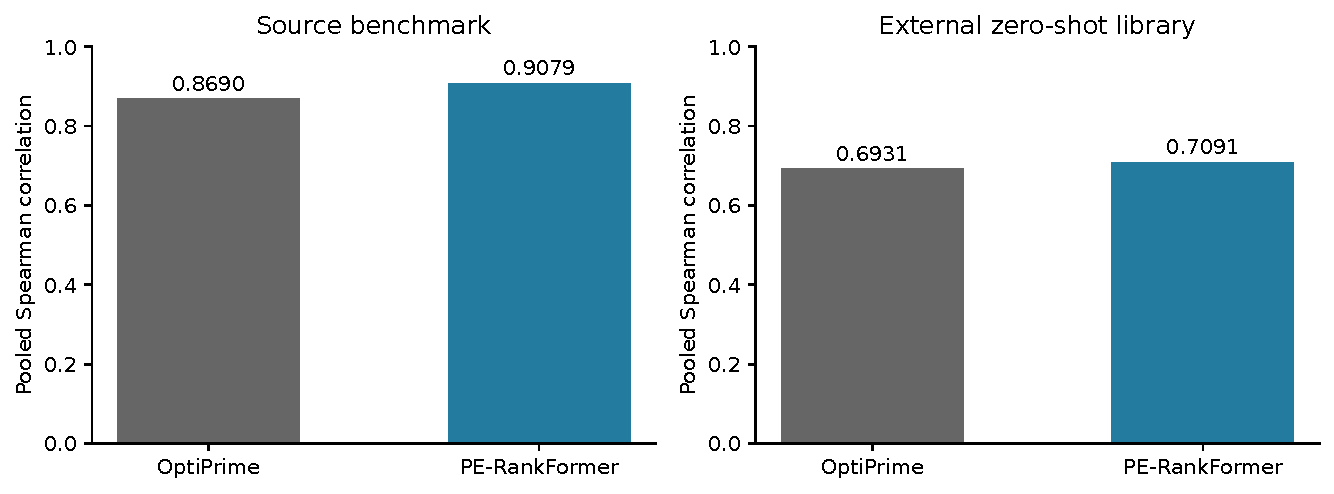
\includegraphics[width=\linewidth]{figures/prediction.pdf}
\caption{\textbf{The ranking advantage extends from the source benchmark to the external library.} Bars show pooled Spearman correlation on the source benchmark and initially reserved external library. The source panel uses the heterogeneous ensemble; the external panel uses its ordinal--S4D member ensembled over five folds. Both comparisons use source-trained models without target-library fine-tuning. Different model configurations and populations preclude interpreting the between-panel change as a controlled estimate of domain shift.}
\label{fig:prediction}
\end{figure}


The ranking advantage also holds within protospacer groups: mean Spearman correlation over 670 eligible groups was $0.6356$ versus $0.5472$, a gain of $0.0884$ (95\% interval $[0.0761,0.1007]$). Because these groups can span edits and conditions, we interpret this as a local ranking endpoint rather than a fixed-edit selection result. Kendall's tau-b increased from $0.6931$ to $0.7478$, with difference $+0.0547$ and interval $[+0.0426,+0.0674]$. Restricting Spearman to positive measured outcomes retained a gain of $+0.0469$ (interval $[+0.0340,+0.0613]$). The improvement therefore extends beyond pooled Spearman and is not explained solely by identifying zero-valued outcomes. Absolute-efficiency calibration and additional robustness checks are reported in Supplementary Sections~\ref{sec:supcalibration} and \ref{sec:suprobust}.

\subsection{The ranking advantage transfers to an external pegRNA library}
We reconstructed the masked edited-sequence representation in the DeepPrime large variant library and removed records sharing the audited protospacer or canonical allele with the source corpus. The resulting panel contains 118,187 measurement rows, corresponding to 118,174 distinct candidates in 30,475 eligible decisions. Unlike the source decision subset, it contains 8,775 groups with at least five candidates and 2,400 with at least eight. Its outcome distribution and PBS/RTT geometry also differ from those of the source benchmark. The initial panel endpoints, grouping and eligibility were declared locally before the original model scoring.


Without target-library training, the ordinal--S4D ensemble achieved pooled Spearman correlation $0.7091$, compared with $0.6931$ for OptiPrime (Figure~\ref{fig:prediction}). This transfer result extends the rank-based advantage beyond the source benchmark, despite changes in candidate depth, PBS/RTT geometry and measured outcome distribution. The external library is a distinct panel from a study also represented in source training; overlap exclusion does not make it an independent-study holdout.

\subsection{Improved source ranking is accompanied by higher top-choice selection efficiency}
We next asked whether improved ranking translates into better pegRNA selection for a fixed intended edit. Canonicalization of the full corpus yielded 51,766 intended alleles and 175,668 allele/context decision groups. The source evaluation fold contains 2,412 groups with at least two distinct candidates, only 85 with at least three, and none with five. Among these, 1,463 groups have nonconstant measured outcomes and support an informative choice. A conventional protospacer grouping instead pools alternatives across conditions and sometimes across desired alleles. We retain within-protospacer correlation as a descriptive statistic, but do not substitute it for the fixed-edit decision endpoint.

On the informative source decisions, the heterogeneous ensemble's top-choice efficiency was $0.13636$ versus $0.12721$ for OptiPrime, a paired gain of $0.00915$ (95\% interval $[0.00633,0.01215]$). Its measured-best-design hit rate was $0.7423$ versus $0.6535$, and regret was $0.00667$ versus $0.01582$. The efficiency gain is a 7.2\% relative improvement, accompanied by an 8.89-percentage-point increase in measured-best-design hit rate. Thus, \model{} improves both overall ordering and the outcome of selecting a single candidate in the source domain. These decisions are predominantly shallow and Kim-derived; they do not establish the same benefit for deeper external candidate sets (Supplementary Table~\ref{tab:decision}).


\subsection{Target-library fine-tuning enables an external selection advantage over OptiPrime}
Native-ordinal fine-tuning provides a second selection-efficiency result, now on the external library (Figure~\ref{fig:selection}; Table~\ref{tab:ordinalselection}).
We next partitioned external-library locus components into adaptation training, validation and test roles. Full-budget fitting used 19,357 training groups, and checkpoint selection used 5,561 validation groups. The retrospective test subset comprised 5,557 groups and 23,044 candidates. The test role prevented direct checkpoint selection on those rows, but this was a repartition of an already studied library, not a new independent study.

Ordinary native-ordinal adaptation achieved mean test utility $0.04178$ over three optimizer seeds, compared with $0.04020$ for released OptiPrime (Table~\ref{tab:ordinalselection}). The gain, approximately $0.00158$ or $0.158$ percentage points of editing efficiency, corresponds to a 3.9\% relative increase and about a 15.7\% reduction in measured oracle regret. Each ordinal seed's paired component interval against OptiPrime was positive. Pooled test Spearman was $0.7771$ versus $0.6922$. This establishes a benefit for target-supervised \model{} relative to the unadapted released comparator, not superiority under equal target-label access.


\begin{table}[htbp]
\centering\small
\caption{Native-ordinal fine-tuning improves external selection over released OptiPrime.}
\label{tab:ordinalselection}
\begin{tabular}{lrrr}
\toprule
Optimizer seed & \model{} $U_1$ & $\Delta$ OptiPrime & Paired 95\% interval \\
\midrule
20260910 & 0.04182 & +0.00162 & $[+0.00094, +0.00227]$ \\
20260911 & 0.04174 & +0.00154 & $[+0.00086, +0.00218]$ \\
20260912 & 0.04178 & +0.00157 & $[+0.00091, +0.00223]$ \\
\bottomrule
\end{tabular}
\par\smallskip
\begin{minipage}{\linewidth}\footnotesize Same retrospective E25 test for every row: 5,557 groups, 23,044 candidates and 4,954 locus components. OptiPrime top-choice efficiency is 0.04020; the mean adapted outcome across seeds is 0.04178. Intervals resample paired locus components conditional on each fitted model, not training seeds or independent studies. All entries are efficiency fractions. Adaptation uses 19,357 training and 5,561 validation groups; OptiPrime receives no target labels.\end{minipage}
\end{table}


\begin{figure}[htbp]
\centering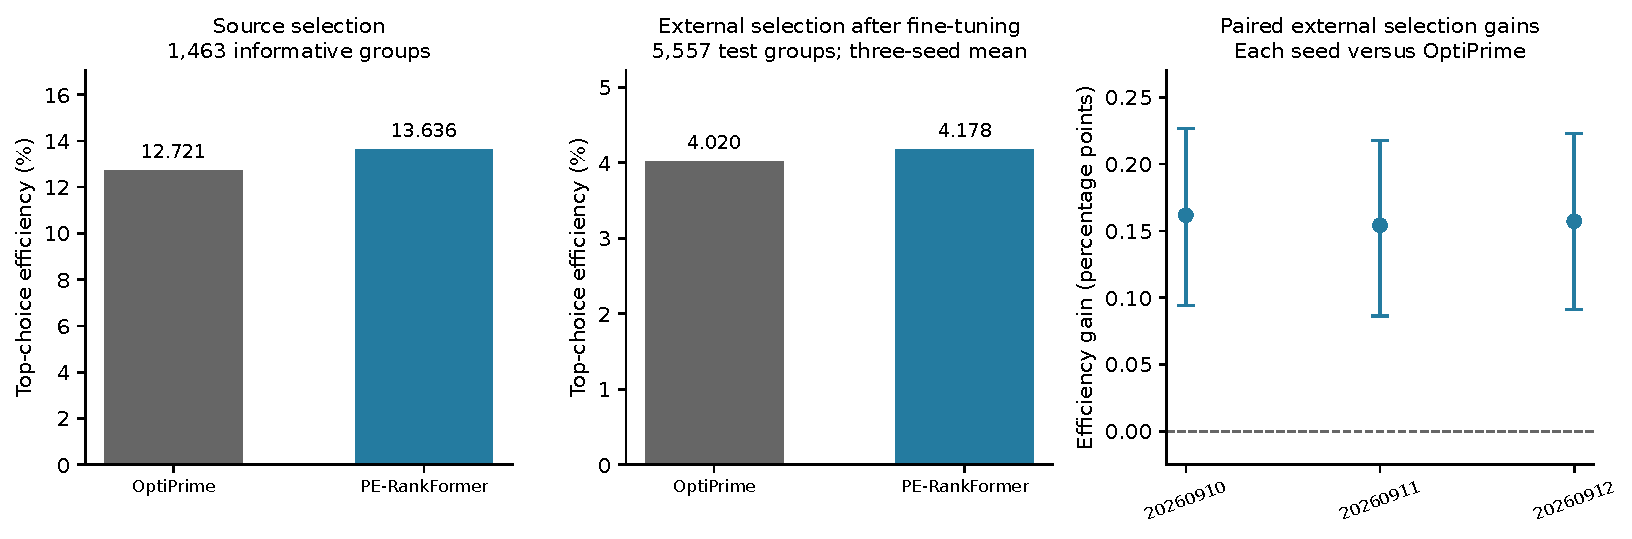
\includegraphics[width=\linewidth]{figures/selection.pdf}
\caption{\textbf{\model{} improves selection in the source domain and after target-library fine-tuning.} Left: source top-choice efficiency over 1,463 informative fixed-edit groups, using the frozen heterogeneous ensemble. Center: retrospective external test efficiency over 5,557 groups, using native-ordinal adaptation (mean outcome across three optimizer seeds). Right: each adapted seed's paired efficiency gain over OptiPrime with its 95\% locus-component bootstrap interval; zero denotes equal top-choice efficiency. The seed intervals condition on the fitted models and are not independent-study replications. The external models use 19,357 training and 5,561 validation groups; released OptiPrime is unadapted. Source and external panels use different populations and model configurations, so their absolute heights are not a paired domain-shift comparison.}
\label{fig:selection}
\end{figure}

Target supervision is an essential condition of the demonstrated external selection advantage. Before fine-tuning, the source-trained ordinal--S4D ensemble's external top-choice efficiency was $0.03627$ versus $0.03690$ for OptiPrime, a difference of $-0.00064$ (95\% interval $[-0.00089,-0.00038]$) on the full 30,475-group panel. Its higher pooled correlation therefore did not by itself guarantee better within-edit selection. Fine-tuned and zero-shot numbers above are evaluated on different denominators; the adaptation result is established by comparing methods on the same 5,557-group test subset, not by subtracting their full-panel and test-subset means. Detailed zero-shot depth-stratified comparisons remain in Supplementary Section~\ref{sec:suptransfer}.

\subsection{Controlled extensions define the supported model and adaptation regime}
Development comparisons support ordinal supervision and S4D within the framework: the retrospective average objective and mixer contrasts in source out-of-fold Spearman were $+0.0092$ and $+0.0192$, respectively. These comparisons are observational rather than a fully matched factorial. Source weighting, ensemble composition and canonical batching also affect results, preventing attribution of the entire OptiPrime margin to one component (Supplementary Sections~\ref{sec:supmodelcontrols} and \ref{sec:supgroupcontrols}).

The native-ordinal fine-tuning result does not depend on a more complex selection head. Separate utility and multitask heads did not establish a replicated additional target advantage, and apparent source retention could disappear when evaluated using their deployed selector instead of an unused prediction head (Supplementary Section~\ref{sec:supheadcontrols}). We therefore emphasize native-ordinal adaptation as the supported procedure for the full-budget selection comparison.

More stringent low-label and source-retention requirements remain unresolved. In the acquisition-replicated, nominal 1,000-group study, neither tuned ordinal adaptation nor source anchoring established a selection win over OptiPrime. A balanced teacher-margin constraint improved retention relative to unconstrained anchoring but sacrificed target utility when source constraints governed checkpoint selection. These results involve an exposed outer development subset and a different label budget, not a refutation or independent confirmation of the full-budget test result (Supplementary Sections~\ref{sec:suplowlabel} and \ref{sec:supretention}). No additional independent-study model evaluation was completed (Supplementary Section~\ref{sec:supdeployment}).
\FloatBarrier
